%%Created by Richard Balson
%%%%%%%%%%%%%%%%%%%%%%%%%%%%%%%%%%%%%%%%%%%%%%%%%%%%%%%%%%%%%

%------------------------------------------------------------
%
\documentclass[10pt]{article}%
%Options -- Point size:  10pt (default), 11pt, 12pt
%        -- Paper size:  letterpaper (default), a4paper, a5paper, b5paper
%                        legalpaper, executivepaper
%        -- Orientation  (portrait is the default)
%                        landscape
%        -- Print size:  oneside (default), twoside
%        -- Quality      final(default), draft
%        -- Title page   notitlepage, titlepage(default)
%        -- Columns      onecolumn(default), twocolumn
%        -- Equation numbering (equation numbers on the right is the default)
%                        leqno
%        -- Displayed equations (centered is the default)
%                        fleqn (equations start at the same distance from the right side)
%        -- Open bibliography style (closed is the default)
%                        openbib
% For instance the command
%           \documentclass[a4paper,12pt,leqno]{article}
% ensures that the paper size is a4, the fonts are typeset at the size 12p
% and the equation numbers are on the left side
%
\usepackage{amsmath}%
\usepackage{amsfonts}%
\usepackage{amssymb}%
\usepackage{graphicx}
\usepackage{hyperref}
\usepackage[round]{natbib}
\usepackage{geometry}
\usepackage{color}
\usepackage{setspace}
\usepackage{pdfsync}
\usepackage{subfig}
\usepackage[export]{adjustbox}
%\usepackage{caption}
%\usepackage{subcaption}
\doublespacing

\def\imagetop#1{\vtop{\null\hbox{#1}}}

%-------------------------------------------
\newenvironment{proof}[1][Proof]{\textbf{#1.} }{\ \rule{0.5em}{0.5em}}

\geometry{top=3cm,bottom=3cm,left=2.5cm,right=3.5cm}

% Text layout
\topmargin 0.0cm
\oddsidemargin 0.5cm
\evensidemargin 0.5cm
\textwidth 16cm 
\textheight 21cm

% Bold the 'Figure #' in the caption and separate it with a period
% Captions will be left justified
\usepackage[labelfont=bf,labelsep=period,justification=raggedright]{caption}

% \newcommand\iref{\textcolor{red}{ref}}
\newcommand\red{\textcolor{red}}

\graphicspath{{fig/}}

\hypersetup{colorlinks,linkcolor=black,filecolor=black,urlcolor=black,citecolor=black} 

\newcommand{\rich}[1]{\textcolor{green}{#1}}
\newcommand{\dean}[1]{\textcolor{blue}{#1}}

\title{Tracking Neural Dynamics: A Model-Based Approach to Demonstrate Variability in Seizures}
\date{\today}
\author{Richard S. Balson, Dean R. Freestone, Mark J. Cook, Anthony N. Burkitt \\ and David B. Grayden}

\begin{document}
\maketitle

\section{Introduction}

\red{Estimate model parameters from a neural mass model of the hippocampus.}

\red{To improve the understanding of epilepsy} 

\red{How has this been achieved previously?}

\red{Introduction to neural mass model, freeman, jansen etc}

\red{What is the output of the model and why}

\red{Is a neural mass model a good model}

\red{Inadequacy of jansen model and intro to the wendling model}

\red{This model is capable of replicating key characteristics observed in EEG prior to and during seizure.}

\red{Is the Wendling model a good model}

\red{Previous work on estimating the neural mass model of the hippocampus has been done using a genetic algorithm.}

\red{Estimation of the neural mass model (Genetic Algorithm)}

\red{Kalman filter}

\red{Why the Kalman filter}

\red{What is being done, and why is it better or different?}

\red{What is being done with the UKF}

\red{Structure of the paper}

\red{Model estimation and accuracy for real data}

\section{Methods}

The purpose of this study is to demonstrate that, using a model-based approach, we can track EEG dynamics in real-time. If we assume that the model we are using is a good model of the system we are recording from, we can then also conclude that the results obtained have physiological meaning, and will allow further insight into the mechanisms involved in seizure generation and termination. We approach the problem of tracking neural dynamics by using two models: an \textsl{in-vivo} model of focal temporal lobe epilepsy with a hippocampal seizure focus and a computational model of the hippocampus.

\subsection{\textsl{In-vivo} Model of Focal Epilepsy}

In this study, we make use of an \textsl{in-vivo} model of focal temporal lobe epilepsy. Epilepsy is induced in rats by injecting tetanus toxin into the CA3 region of their hippocampus~\citep{jefferys1995chronic}. This model has a localised seizure focus, and results in seizure events that are similar to the electrophysiological and physical symptoms observed in human patients with temporal lobe epilepsy. 

Sprague Dawley rats~(300-400 grams) are injected with $0.4-0.6\mu l$ of tetanus toxin. The tetanus toxin is injected into the CA3 region of the left hippocampus - $-3.5mm$ anterior-posterior (AP), $3mm$ medial lateral and $-3.5mm$ dorsal ventral (DV), relative to bregma. Four electrodes are placed to record local field potentials: a twisted pair electrode is inserted into the same location as the tetanus toxin, and two screw electrodes are placed on the surface of the cortex on the right hemisphere. A cerebellar electrode is placed as a reference for all electrodes. Electrodes are connected to a pedestal and held in place by dental cement. The animals are left to recover for five to seven days, and are recorded from for 24 hours a day for six to eight weeks.\footnote{For some animals shorter durations of recordings are obtained due to pedestals failure.} All experiments are done under the approval of an ethics committee.

\subsection{Neural Mass Model} 

All neural field models can be described by a temporal and spatial response curve, and a function that relates membrane potentials to firing rates. For neural mass models the spatial element is assumed to be constant due to the cortical area considered being small. The general description can therefore be described by a convolution integral over time,

\begin{equation}\label{eq:conv_eq}
    v_n(t) = \frac{\alpha_{mn}}{\tau_{mn}}\int_{-\infty}^t  h_{mn}(t-t')g(v_m(t')) \,\mathrm{d}t' + v_r,
\end{equation}
where $\alpha_{mn}$ is a lumped parameters specifying the connectivity and synaptic strength between populations $m$ and $n$ as well as the maximal firing rate of population $m$, $h_{mn}(t)$ is the temporal response curve - commonly referred to as a post synaptic response kernel. The time constant $\tau_{mn}$  describes the average delay between the time population $m$ produces a firing rate and the time population $n$ receives the maximal potential due to the firing rate. The effect of the resting membrane potential on the model is specified by $v_r$. The temporal response curve (Figure~\ref{fig: Simple}) is a time delayed exponential decay function:
\begin{equation}
    h_{mn}(t) = \eta(t)t\exp\left(-\frac{t}{\tau_{mn}}\right),
\end{equation}
where $\eta(t)$ is the Heaviside step function. 

\begin{figure}
	\centering
		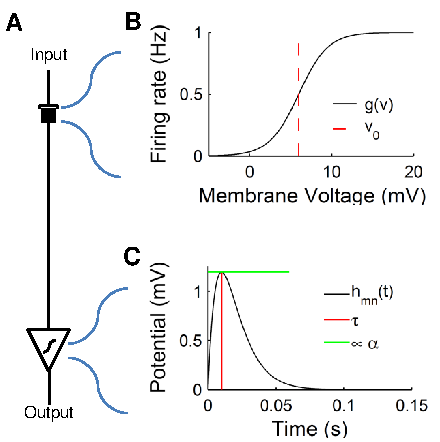
\includegraphics{Biological_Response.pdf}
	\caption{Simple Neural Mass Model. (\textbf{A}) An example of a simple neural mass model. This model consists of a single neural population - the triangle - and a single synapse - the square block. (\textbf{B}) Temporal response curve for a synapse. The black line demonstrates the response of a synapse to a firing rate. The time constant ($\tau$) and synaptic gain ($\alpha$) are demonstrated in this figure. The peak response of this function is $\alpha \exp(-1)$ and the time at which this peak occurs is $\tau$. (\textbf{C}) Somatic response curve. The black line indicates the function $g(v)$, a sigmoid. This function demonstrates the resulting normalized firing rate produced by a neural population as a function of the membrane potential over it. In this figure $v_{0}$ is the membrane potential at which the firing rate produced is half its maximum.}
	\label{fig: Simple}
\end{figure}

The firing rate of each population is determined from a sigmoid function~(Figure~\ref{fig: Simple}), that models the action of a specific population's somas. The sigmoid function translates the membrane potential of a population to its aggregate firing rate,
\begin{align}\label{eq:sigmoid}
    g\left(v_n(t)\right) =& \frac{1}{1+\exp{\left(\varsigma_n\left(v_{0n} - v_n(t)\right)\right)}}.
\end{align}
The quantity $\varsigma_n$ describes the gradient of the sigmoid activation curve and $v_{0n}$ the membrane potential that results in half the maximum firing rate. The constant $v_{0n}$ is a lumped parameter, that includes the effect of the resting membrane potential on the activation curve. 

The convolution integral in Equation~\ref{eq:conv_eq} can be written as an ordinary differential equation (ODE)
\begin{equation}\label{eq:2ndOrder}
    \mathrm{D}v_n(t) = \frac{\mathrm{d}^2 v_n(t)}{\mathrm{d}t^2} + \frac{2}{\tau_{mn}}\frac{\mathrm{d} v_n(t)}{\mathrm{d}t} + \frac{1}{\tau_{mn}^2} v_n(t) = \frac{\alpha_{mn}}{\tau_{mn}} g(v_m(t)),
\end{equation}
where $\mathrm{D}$ is a differential operator. Equation~\ref{eq:2ndOrder} can also be written as a pair of coupled partial differential equations
\begin{equation} \label{eq:2ndOrderNMM}
    \frac{\mathrm{d} v_n(t)}{\mathrm{d}t} = z_n(t),\,\,\,\,\,    \frac{\mathrm{d}z_n(t)}{\mathrm{d}t} = \frac{\alpha_{mn}}{\tau_{mn}} g(v_m(t)) - \frac{2}{\tau_{mn}}z_n(t) - \frac{1}{\tau_{mn}^2} v_n(t),
\end{equation}
where $z_n(t)$ is the time derivative of $v_n(t)$. These two partial differential equations form the basis of a state-space model for all neural masses.

The simplest possible neural mass model has a single population with a single input and output firing rate~(Figure~\ref{fig: Simple}). This model consists of a single post synaptic response curve and a sigmoid function.

In this study, we consider the neural mass model of the hippocampus (Figure~\ref{fig: Biological}). This is an expansion of the simple model (Figure~\ref{fig: Simple}) where four populations - two excitatory and two inhibitory - are included. Each populations post synaptic response curve is described by a time constant ($\tau_{mn}$) and synaptic response ($\alpha_{mn}$). Here we make the assumption that the time constants of all the populations are static (Table~\ref{tab: Static}) and that the synaptic responses are time varying. This assumption allows the computational model we are considering to mimic EEG recorded from the hippocampus by varying the fewest number of model parameters. This assumption also implies that the synapse are current, rather than conductance, based. The synaptic responses are a lumped term
\begin{equation}\label{eq: Synaptoic response}
    \alpha_{\mathrm{mn}} = 2\epsilon_{0}c_{mn}\theta_{mn},
\end{equation} where $\epsilon_0$ is half the maximum firing rate of population $m$, $c_{mn}$ is the number of synaptic connections between population $m$ and $n$ and $\theta_{mn}$ is the synatpic gain of the synapse between population $m$ and $n$. The input to the model represents the firing rate from the rest of the brain to the modeled population, and is modeled as a Gaussian noise source with a non-zero mean.

We assume that all excitatory temporal response curves have the same synaptic gain, that is:
\begin{equation}\label{eq:ExcSynapse}
    \theta_{\mathrm{pe}} = \theta_{\mathrm{ps}} = \theta_{\mathrm{pf}} = \theta_{\mathrm{ep}} = \theta_{\mathrm{ip}},\,\,\,\,\, \tau_{\mathrm{pe}} = \tau_{\mathrm{ps}} = \tau_{\mathrm{pf}} = \tau_{\mathrm{ep}} = \tau_{\mathrm{ip}},
\end{equation} where the subscripts represent the pyramidal (p), excitatory (e), slow inhibitory (s) and fast inhibitory (f) populations and the model input (i). For simplicity the synaptic gains and time constants of all excitatory populations will be described by $\theta_{\mathrm{p}}$ and $tau_{\mathrm{p}}$. With this assumption the synaptic response of different synapses can be related to each other by
\begin{equation}\label{eq:ExcSynapseResp}
    \theta_{\mathrm{p}} = \frac{\alpha_{\mathrm{pe}}}{2\epsilon_{0}c_{\mathrm{pe}}}=\frac{\alpha_{\mathrm{ps}}}{2\epsilon_{0}c_{\mathrm{ps}}}=\frac{\alpha_{\mathrm{pf}}}{2\epsilon_{0}c_{\mathrm{pf}}}=\frac{\alpha_{\mathrm{ep}}}{2\epsilon_{0}c_{\mathrm{ep}}}=\frac{\alpha_{\mathrm{ip}}}{2\epsilon_{0}c_{\mathrm{ip}}},
\end{equation} 
 The same assumption is also made for the slow inhibitory temporal response curves
		\begin{equation}\label{eq:InhSynapse}
		\theta_{\mathrm{sf}} = \theta_{\mathrm{sp}},\,\,\,\,\, \tau_{\mathrm{sf}} = \tau_{\mathrm{sp}}.
\end{equation} For simplicity the synaptic gain and time constants of the slow inhbitiory synapses will be referred to by $\theta_{\mathrm{s}}$ and $\tau_{\mathrm{s}}$ and the synaptic responses can be related by
 \begin{equation}\label{eq:InhSynapseResp}
    \theta_{\mathrm{s}} = \frac{\alpha_{\mathrm{sf}}}{2\epsilon_{0}c_{\mathrm{sf}}}=\frac{\alpha_{\mathrm{sp}}}{2\epsilon_{0}c_{\mathrm{sp}}}
\end{equation} 
By making this assumption we can reduce the number of synapse required to model this neural mass (Figure~\ref{fig: Biological}), while retaining all the dynamics in the model required to mimic recorded hippocampal EEG. As a last simplification we describe the fast inhibitory synaptic gain by $\theta_{\mathrm{f}}$ and $\tau_{\mathrm{f}}$. 

In this study we estimate the synaptic gains~($\theta$) of the three types of synapses as well as the mean input firing rate. All other parameters are considered to be static (Table~\ref{tab: Static}).

\singlespacing 
\footnotesize
\begin{center}%%%%%%%%%%%%%%%%%%%%%%%%%%%%%%%%%%%%%%%%%%
	\begin{table}
			\caption{Static Model Parameters~\citep{wendling2002epileptic}. Here p, e, s and f represent populations of pyramidal neurons and excitatory, and slow and fast inhibitory interneurons, respectively.}
		\begin{tabular}{||p{2.5cm}|p{9cm}|p{1.2cm}|p{1cm}||}\hline
			 \textsc{Parameter}  & \textsc{Physical description} & \textsc{Value} & \textsc{Units}  \\\hline\hline
			 $\tau_{\mathrm{p}}$ & Time constant for excitatory temporal response curve & 100 & $s^{-1}$\\\hline
			 $\tau_{\mathrm{s}}$ & Time constant for slow inhibitory temporal response curve & 35 & $s^{-1}$\\\hline
			 $\tau_{\mathrm{f}}$ & Time constant for fast inhibitory temporal response curve & 500 & $s^{-1}$\\\hline
			 $C$ & Connectivity scale & 135 & NA\\\hline
			 $c_{\mathrm{pe}}$ & Connectivity constant  & $C$ & NA \\\hline
			 $c_{\mathrm{ep}}$ & Connectivity constant  & $0.8C$ & NA\\\hline
			 $c_{\mathrm{ps}}$ & Connectivity constant  & $0.25C$ & NA \\\hline
			 $c_{\mathrm{sp}}$ & Connectivity constant  & $0.25C$ & NA\\\hline
			 $c_{\mathrm{pf}}$ & Connectivity constant  & $0.3C$ & NA\\\hline
			 $c_{\mathrm{sf}}$ & Connectivity constant  & $0.1C$ & NA\\\hline
			 $c_{\mathrm{fp}}$ & Connectivity constant  & $0.8C$ & NA\\\hline
			 $\epsilon_{0}$ & 50\% of maximum firing rate & 2.5 & Hz \\\hline
			 $v_{0}$ & Membrane potential resulting in 50\% of maximal firing rate & 6 & $mV^{-1}$\\\hline
			 $\varsigma$ & Gradient of sigmoid function & 0.56 & NA \\\hline
		\end{tabular}
		\label{tab: Static}
	\end{table}
\end{center}%%%%%%%%%%%%%%%%%%%%%%%%%%%%%%%%%%%%%%%%%%%%%%%%%%%%%%%%%%
\doublespacing
\normalsize

 \begin{figure}
 	\centering
 		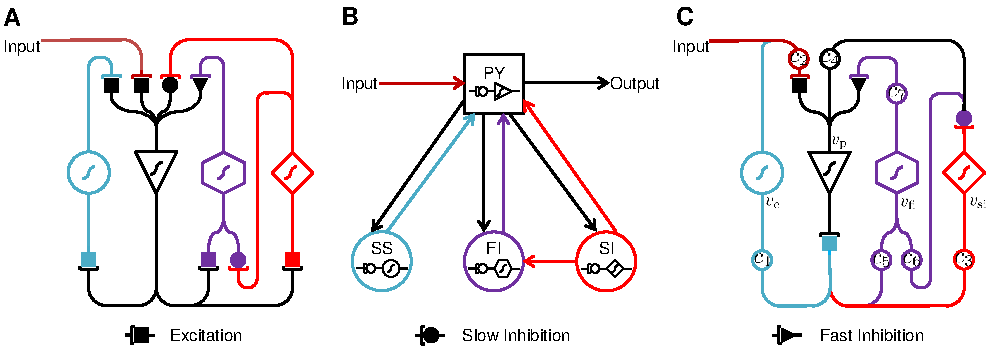
\includegraphics{fig/Biological_Model.pdf}
 	\caption{Graphical Description and Simplification of the Neural Mass Model of the Hippocampus. (\textbf{A}) Graphical description of the neural mass model of the hippocampus. In this figure the traingle, circle, diamond and hexagon represent populations of pyramidal (PY), spiny stellate (SS) and slow (SI) and fast inhibitory (FI) neurons. Synapses are specified by a u shaped structure, where the secondary terminal has different shapes depending on the type of synapse. The model input is a firing rate from other cortical regions connected to the modeled area. (\textbf{B}) Flow diagram of the neural mass model of the hippocampus. (\textbf{C}) Simplified graphical description of the neural mass model of the hippocampus.}
 	\label{fig: Biological}
 \end{figure}


\subsection{Estimation}

\red{Generic description of a nonlinear system}

We begin by defining a generic non-linear system\begin{align}
\label{eqn: NonlinEstS}
\mathbf{\dot{x}}(t) &= \mathbf{A}(\mathbf{x}(t),\mathbf{\theta}(t)) + \mathbf{B}(\mathbf{u}(t)) + \mathbf{n}(t)\\
\label{eqn: NonlinEstO}
\mathbf{y}(t)  &= \mathbf{C}(\mathbf{x}(t)) +\mathbf{D}(\mathbf{u}(t))+\mathbf{r}(t),
\end{align} where boldface is used to indicate a matrix or vector. For a non-linear system boldface notation can also indicate a matrix of functions. Here, $\mathbf{x}(t)$ is the model states and $\dot{\mathbf{x}}(t)$ its derivative, where
\[ \mathbf{\dot{x}}(t) = \left[ \begin{array}[pos]{c}
\dot{x}_{1}(t)\\
\vdots \\
\dot{x}_{n}(t) \end{array} \right] .\] The state and input matrices are $\mathbf{A}$ and $\mathbf{B}$, respectively and $\mathbf{u}(t)$ is the model input. The observation and input-to-output matrices are $\mathbf{C}$ and $\mathbf{D}$, respectively. The output and uncertainty of the model are $y(t)$ and $n(t)$, with $\mathbf{r}(t)$ the observation noise. Both $\mathbf{n}(t)$ and $\mathbf{r}(t)$ are zero mean Gaussian distributed with a system dependant variance. 


\red{Introduction to the UKF}

Estimation techniques attempt to approximate model states given some observation. There are numerous techniques to achieve this, most of which are for linear systems. We make use of a nonlinear estimation technique, the unscented Kalman filter. The filter consists of two steps: prediction and correction. In the prediction step an unscented transform~(Figure~\ref{fig: UKF}) is used to approximate the mean and covariance of states after they have been propagated through the model. The correction step uses this prediction to determine the most likely states, given the observation from the system. The correction step makes use of the uncertainty on both the observations and the states to determine how they are weighted for the corrected estimate~(Figure~\ref{fig: UKF}).

The unscented transform makes the assumption that the distribution of states before and after they are propagated through the model can be described by a Gaussian distribution~(Figure~\ref{fig: UKF}). The first step in the unscented transform is the extraction of sigma points - points one standard deviation away from the mean, 
\begin{align}\label{eqn: SigmaP}
\mathbf{\mathcal{X}}_{0} &= \mathbf{\overline{x}}_{k} \quad iff \quad \kappa >0\\
\mathbf{\mathcal{X}}_{n,k} &= \mathbf{\overline{x}}_{k} + (\sqrt{\kappa+D_{x}\mathbf{P_{xx,k}}})_{n} \quad n=1,\hdots,D_x,\\
\mathbf{\mathcal{X}}_{n+D_x,k} &= \mathbf{\overline{x}}_{k} - (\sqrt{\kappa+D_{x}\mathbf{P_{xx,k}}})_{n} \quad n=1,\hdots,D_x,
\end{align} where $\mathbf{\mathcal{X}}_{n}$ are the sigma points, $k$ the current sample, $\mathbf{\overline{x}}_{k}$ and $\mathbf{P_{xx,k}}$ are the states expected value and covariance and $D_{x}$ is the dimensionality of the system. There are $2D_x$ or $2D_{x}+1$ sigma points depending on the value of $\kappa$. In general, the value of $\kappa$ is used to either scale up or scale down the effect of the mean on the unscented transform prediction. Here we assume that $\kappa$ is greater than zero for the derivation of the unscented Kalman filter. The notation $\sqrt{\cdot}_{n}$ is used to indicate the $n$th row of the matrix square root. 

Next, the sigma point are propagated through the model, and the results are used to evaluate the statistics of the prediction,
\begin{align}\label{eqn: SigmaProp}%%%%%%%%%%%%%%%%%%%%%%%%%%%%%%%%%%%%
\mathbf{\mathcal{X}}_{n,k+1} &= \mathbf{\mathcal{X}}_{n,k}+ T(\mathbf{A}(\mathbf{\mathcal{X}}_{n,k}) +\mathbf{B}(\mathbf{u}_{k})),\\
\label{eqn: PriorSMean}
\overline{\mathbf{x}}_{k+1}^{-} &= \frac{1}{2D_{x}+\kappa}\sum_{n=0}^{2D_{x}} \mathbf{\mathcal{X}}_{n,k+1},\\
\label{eqn: PriorSCov}
\mathbf{P}_{xx,k+1}^{-} &= \frac{1}{2D_{x}+\kappa}\sum_{n=0}^{2D_{x}} (\mathbf{\mathcal{X}}_{n,k+1} -\mathbf{\overline{x}}_{k+1}^{-})(\mathbf{\mathcal{X}}_{n,k+1}-\mathbf{\overline{x}}_{k+1}^{-})^{\top} + \mathbf{Q},%%%%%%%%%%%%%%%%%%%%%%%%%%%%%%%%%%%%
\end{align} $\mathbf{\mathcal{X}}_{n,k+1}$ are the propagated sigma points, $\overline{\mathbf{x}}_{k+1}^{-}$ and $\mathbf{P}_{xx,k+1}^{-}$ are the predictions for the states and their covariances. The negative superscript is used to indicate an uncorrected prediction. The term $\mathbf{Q}$ is the covariance of $\mathbf{n(t)}$ and $(\cdot)^{\top}$ a matrix transpose. In this step, a first order Euler approximation is used to propagate the model states one sample forward. This involves scaling the propagation by the sampling period ($T$).

Using equations~\ref{eqn: SigmaProp}-\ref{eqn: PriorSCov} a prediction about the next observation can be made. The neural mass model's observation function is linear; therefore, the statistics of the observation can be determined from the propagated sigma points,
\begin{align}
\mathbf{\mathcal{Y}}_{n,k+1} &= \mathbf{C}(\mathbf{\mathcal{X}}_{n,k+1})+ \mathbf{D}(\mathbf{u}_{k})\\
\overline{\mathbf{y}}_{k+1}^{-} &= \frac{1}{2D_{x}+\kappa}\sum_{n=0}^{2D_{x}} \mathbf{\mathcal{Y}}_{n,k+1}\\
\label{eqn: statecovg}
\mathbf{P}_{xy,k+1}^{-} &= \frac{1}{2D_{x}+\kappa}\sum_{n=0}^{2D_{x}} (\mathbf{\mathcal{X}}_{n,k+1}-\overline{\mathbf{x}}_{n,k+1}) (\mathbf{\mathcal{Y}}_{n,k+1}-\overline{\mathbf{y}}_{k+1}^{-})^{\top}\\
\mathbf{P}_{yy,k+1}^{-} &= \frac{1}{2D_{x}+\kappa}\sum_{n=0}^{2D_{x}} (\mathbf{\mathcal{Y}}_{n,k+1}-\overline{\mathbf{y}}_{k+1}^{-}) (\mathbf{\mathcal{Y}}_{n,k+1}-\overline{\mathbf{y}}_{k+1}^{-})^{\top} +\mathbf{R},%%%%%%%%%%%%%%%%%%%%%%%%%%%%%%%%%%%%%%%%%%%%
\end{align} where $\mathbf{\mathcal{Y}}_{n,k+1}$ are the predicted observations from all the sigma points, and $\overline{\mathbf{y}}_{k+1}^{-}$ and $\mathbf{P}_{yy,k+1}^{-}$ are the predictions for the model output and its covariance, respectively. The covariance matrix of the states and observations are $\mathbf{P}_{xy,k+1}^{-}$ and $\mathbf{R}$ is the covariance of the observation error $\mathbf{r(t)}$.

In the correction step the covariance and predicted observation is compared to the recording from the system. This comparison puts more weight on the value with the lowest covariance, and adjusts the value of the predicted states accordingly. This is achieved using the standard formulation of the Kalman filter correction step,
\begin{align}
\mathbf{K} &= \mathbf{P}_{xy,k+1}^{-}(\mathbf{P}_{yy,k+1}^{-})^{-1}\\
\overline{\mathbf{x}}_{k+1} &= \overline{\mathbf{x}}_{k+1}^{-} + \mathbf{K}(\mathbf{y}_{k+1}-\overline{\mathbf{y}}_{k+1}^{-})\\
\mathbf{P}_{xx,k+1} &= \mathbf{P}_{xx,k+1}^{-} - \mathbf{K}(\mathbf{P}_{xy,k+1}^{-})^{\top},
\end{align} where $\mathbf{K}$ is the Kalman gain, $\mathbf{y}_{k+1}$ is the observation, $\overline{\mathbf{x}}_{k+1}$ is the corrected estimate of the state and $\mathbf{P}_{xx,k+1}$ its covariance.

 \begin{figure}
 	\centering
 		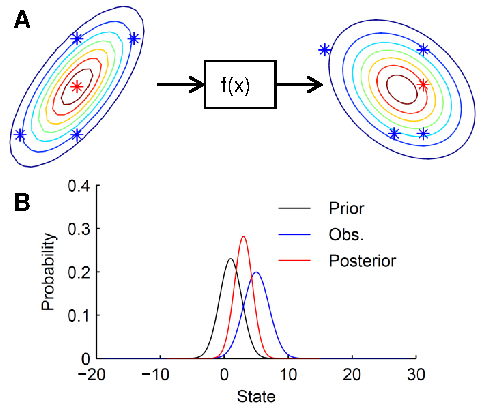
\includegraphics{fig/UnscentedKalman.pdf}
 	\caption{The unscented Kalman filter. (\textbf{A}) The unscented transform. In this figure the a Gaussian distribution of a two dimensional state space is shown. Points one standard deviation  from the mean (red star) are drawn from this distribution (blue stars) and propagated through the system ($f(x)$). The resulting points and the estimated Gaussian distribution of the states is then approximated. (\textbf{B}) The Kalman filter. The prior distribution in the figure is the result from the unscented transform. The Kalman filter predicts the most likely state (Posterior) and its expected error making use of the knowledge of the distributions of the predicted state from the unscented transform and the observation (Obs.). This result is then used in the next iteration of the unscented transform.}
 	\label{fig: UKF}
 \end{figure}


%\red{Definition of slow state matrix and its dynamics}

In this paper we are interested in estimating aspects of physiology that are unobserved by making use of a neural mass model. In particular, we consider the estimation of the model's synaptic gains ($\theta$). To estimate model parameters they need to be augmented to the original models state matrix, 
\[ \mathbf{\dot{x}}(t) = \left[ \begin{array}[pos]{c}
\dot{x}_{1}(t)\\
\vdots \\
\dot{x}_{n}(t)\\
\dot{\theta}_{1}(t)\\
\vdots\\
\dot{\theta}_{n}(t) \end{array} \right] .\] Here $\theta_{1-n}$ are the model parameters that are estimated, and are assigned trivial dynamics,
\begin{equation}\label{eq: ParameterDyn}
 \mathbf{\dot{\theta}}=0,
\end{equation}
The model parameters can be assigned trivial dynamics due to the prediction correction nature of the unscented Kalman filter. Model parameters are assumed to be constant with some error assigned to them. The error assigned to each parameter allows the correction step of the unscented Kalman filter deytermine the most likely set of parameters that describe the current observation. This technique allows the model parameters to slowly vary with each observation made. The change in model parameters occurs at a longer time scale than the model states; Therefore, for convenience, the model states and parameters are referred to as fast and slow states, respectively. 

As a further addition, the mean input firing rate to the modeled cortical region as a slowly state. This addition allows us to estimate the effect of other cortical regions on the seizure focus during the transition to seizure.

In the results section we demonstrate three key components for any estimation procedure using computational models: model selection and fitting, and estimation validation. To demonstrate that the computational model, and all the assumptions made, are descriptive of the type of data we are considering a comparison between the model output and recorded EEG is made. Following this, we fit the synaptic gains and input mean of the computational model to the recorded data. Lastly, we use the estimated model parameters to simulate EEG using the computational model. We then compare the characteristics of the simulated EEG to the recorded data from the \textsl{in-vivo} model.



\section{Results}





%\section{Discussion}



%\red{Why estimation}
%
%\red{Effect of stochastic input}
%
%\red{Estimation of model parameters}
%
%\red{Initialisation error}
%
%\red{Observation Noise}
%
%\red{Parameters varying}
% 
% \section{Discussion}


% 
% \section{Conclusion}

In this paper we have demonstrated that the tracking of neural dynamics using an unscented Kalman filter is feasible. We have also shown that there are clear differences between the mechanisms involved in seizure initiation and termination between and in some cases within animals. This information could be used to help with the development of new therapies. Some of the aspects that were not discussed in this paper include variability due to severity of seizures, and the long term evolution of seizures in an animal model where seizure frequency decreases over time. 
% 
% \section{Appendix}
\label{sec: AppendixA}

The reduction of the Wendling model is based on the principles of linear superposition. First notice that each synapse is a linear lowpass filter (equation~\ref{eqn: LaplaceNMM}). In figure~\ref{fig: Biological} there are eight such synapse. However, notice that numerous of these synapse have identical synaptic gains, and are connected by different connectivity constants. Given that for a linear system it is known that
\begin{align}
f(a\mathbf{x}) = af(\mathbf{x}),
\end{align} where $f(\cdot)$ is an arbitrary function, and $a$ is a constant. Therefore, the model can be simplified by moving the synapse closer to the respective populations. The result of this process is demonstrated in figure~\ref{fig: BiologicalMin}.

\begin{figure}  %%%%%%%%%%%%%%%%%%%%%%%%%%%%%%%%%%%%%%%
	\centering
		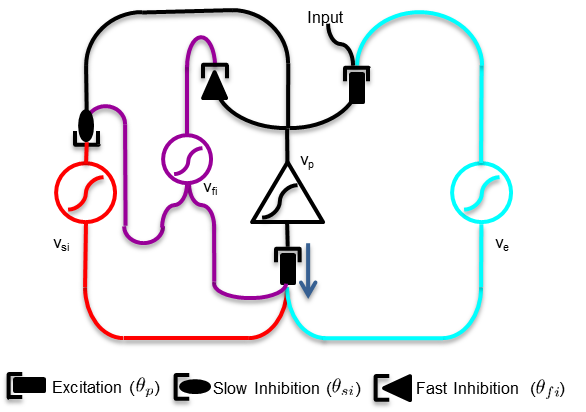
\includegraphics{Biological_Model_DescriptionMin.png}
	\caption{Graphical Description of the Wendling model (Minimised). Membrane potentials are shown and named $v_{b}$ where $b$ is $p$, $e$, $fi$ and $si$ for pyramidal, excitatory and slow and fast inhibitory populations, respectively. The synaptic gains of each population are specified by $\theta_{m}$ where $m$ is defined in the same manner as the membrane potentials and $\theta_{p}=\theta_{e}$. Each triangle and circle indicates a neural population. In particular, the triangle shape indicates the pyramidal population and the circle shapes represent interneurons. The triangles and circles model the action of the soma for the neural populations, and convert membrane potentials to firing rates. The synapses convert the firing rates to membrane potentials. Lastly, each line indicates a neural connection, which is specified by a connectivity constant.}
	\label{fig: BiologicalMin}
\end{figure}%%%%%%%%%%%%%%%%%%%%%%%%%%%%%%%%%%%%%%%%%%%%%

Now consider the full set of original model equations that would be required to specify figure~\ref{fig: Biological}
\begin{align}
\label{eqn: Fullmodel Descrip}
\mathrm{d}v_{po*}(t)&= z_{po*}(t)\mathrm{d}t\\
\mathrm{d}z_{po*}(t)&=\left(\frac{\theta_{p}(t)}{\tau_{p}}c_{1}g(v_{p}(t))-2\frac{z_{po*}(t)}{\tau_{p}}-\frac{v_{po*}(t)}{\tau_{p}^{2}}\right)\mathrm{d}t\\
\mathrm{d}v_{p1*}(t)&= z_{p1*}(t)\mathrm{d}t\\
\mathrm{d}z_{p1*}(t)&=\left(\frac{\theta_{p}(t)}{\tau_{p}}c_{3}g(v_{p}(t))-2\frac{z_{p1*}(t)}{\tau_{p}}-\frac{v_{p1*}(t)}{\tau_{p}^{2}}\right)\mathrm{d}t\\
\mathrm{d}v_{p2*}(t)&= z_{p2*}(t)\mathrm{d}t\\
\label{eqn: Pyr}
\mathrm{d}z_{p2*}(t)&=\left(\frac{\theta_{p}(t)}{\tau_{p}}c_{5}g(v_{p}(t))-2\frac{z_{p2*}(t)}{\tau_{p}}-\frac{v_{p2*}(t)}{\tau_{p}^{2}}\right)\mathrm{d}t\\
\label{eqn: SI}
\mathrm{d}v_{p3*}(t)&= z_{p3*}(t)\mathrm{d}t\\
\mathrm{d}z_{p3*}(t)&=\left(\frac{\theta_{si}(t)}{\tau_{si}}c_{4}g(v_{si}(t))-2\frac{z_{p3*}(t)}{\tau_{si}}-\frac{v_{p3*}(t)}{\tau_{si}^{2}}\right)\mathrm{d}t\\
\mathrm{d}v_{p4*}(t)&= z_{p4*}(t)\mathrm{d}t\\
\label{eqn: SI1}
\mathrm{d}z_{p4*}(t)&=\left(\frac{\theta_{si}(t)}{\tau_{si}}c_{6}g(v_{si}(t))-2\frac{z_{p4*}(t)}{\tau_{si}}-\frac{v_{p4*}(t)}{\tau_{si}^{2}}\right)\mathrm{d}t\\
\label{eqn: FI}
\mathrm{d}v_{p5*}(t)&= z_{p5*}(t)\mathrm{d}t\\
\label{eqn: FI2}
\mathrm{d}z_{p5*}(t)&=\left(\frac{\theta_{fi}(t)}{\tau_{fi}}c_{7}g(v_{fi}(t))-2\frac{z_{p4*}(t)}{\tau_{fi}}-\frac{v_{p5*}(t)}{\tau_{fi}^{2}}\right)\mathrm{d}t\\
\label{eqn: Exc}
\mathrm{d}v_{p6*}(t)&= z_{p6*}(t)\mathrm{d}t\\
\mathrm{d}z_{p6*}(t)&=\left(\frac{\theta_{e}(t)}{\tau_{e}}c_{2}g(v_{e}(t))-2\frac{z_{p6*}(t)}{\tau_{e}}-\frac{v_{p6*}(t)}{\tau_{e}^{2}}\right)\mathrm{d}t\\
\mathrm{d}v_{p7*}(t)&= z_{p7*}(t)\mathrm{d}t\\
\label{eqn: WienerFull}
\mathrm{d}z_{p7*}(t)&=\left(\frac{\theta_{p}(t)}{\tau_{p}}\mu -2\frac{z_{p7*}(t)}{\tau_{e}}-\frac{v_{p7*}(t)}{\tau_{p}^{2}}\right)\mathrm{d}t + \frac{\theta_{p}(t)}{\tau_{p}}\epsilon(t)\mathrm{d}W.\\
\end{align} In these equations $dW$ represents a Wiener process and is required as $\epsilon(t)\sim N(0,\sigma)$, where $\sigma$ and $\mu$ (equation~\ref{eqn: Wiener}) describe the mean and variance of the stochastic model input. Further, $v_{po}(t) $ and $v_{p1-7*}(t)$ represent the membrane potential produced by each synapse and $z_{po*}(t) $ and $z_{p1-7*}(t)$ their derivatives. The inputs to each neural population are specified by $v_{b}(t) $ and $z_{b}(t) $, and are the membrane potential of the specific population, where $b$ takes the values of $p$, $e$, $fi$ and $si$ representing pyramidal, excitatory, and slow and fast inhibitory populations, respectively. Therefore $v_{p}(t) $ is the output of the model. All $v_{b}(t) $ can be described in terms of $v_{po}(t)$ and $v_{p1-7}(t)$ as follows
\begin{align}
\label{eqn: pop1}
v_{p}(t) &= v_{p6*}(t)+v_{p7*}(t)-v_{p3*}(t)-v_{p5*}(t)\\
\label{eqn: pop2}
v_{e}(t) &= v_{po*}(t)\\
\label{eqn: pop3}
v_{si}(t) &= v_{p1*}(t)\\
\label{eqn: pop4}
v_{fi}(t) &= v_{p2*}(t)-v_{p4*}(t).
\end{align} Notice that equations~\ref{eqn: Fullmodel Descrip}-\ref{eqn: Pyr} and equations~\ref{eqn: SI}-\ref{eqn: SI1} are identical except for the connectivity constants. Further, in this model it is assumed that 
\begin{align}
\theta_p = \theta_e\\
\tau_p = \tau_e.
\end{align} Therefore, equations~\ref{eqn: Exc}-\ref{eqn: WienerFull} are identical, but have different inputs. Next consider the effect of the states $v_{p0-7*}(t)$ and $z_{p0-7*}(t)$ on the model inputs. Note that since the effect of $v_{p6*}(t)$ and $v_{p7*}(t)$ are additive, they can be added prior to being passed through the linear filter since
\begin{align}
f{x} + f{y} = f{x+y},
\end{align} where f is defined above and $x$ and $y$ are arbitrary variables. Therefore equations~\ref{eqn: Exc}-\ref{eqn: WienerFull} can be simplified to the following:
\begin{align}
\mathrm{d}v_{p1}(t)&= z_{p1}(t)\mathrm{d}t\\
\label{eqn: Wiener1}
\mathrm{d}z_{p1}(t)&=\left(\frac{\theta_{e}(t)}{\tau_{e}}(\mu +n_{e}g(v_{e}(t))-2\frac{z_{p1}(t)}{\tau_{e}}-\frac{v_{p1}(t)}{\tau_{e}^{2}}\right)\mathrm{d}t + \frac{\theta_{e}(t)}{\tau_{e}}\epsilon(t)\mathrm{d}W.
\end{align}. By making this reduction the effect of both the excitatory population and the input have been incorporated in one potential. Therefore, $v_{p7*}(t)$ is no longer required in equations~\ref{eqn: pop1}. 

Next consider the equations that only have connectivity constants that are different. Notice that these connectivity constants scale the input to the function, and this scaling can be performed after the input is transformed by the linear function. Therefore, equations~\ref{eqn: Fullmodel Descrip}-\ref{eqn: Pyr} can be represented by a single equation such that
\begin{align}
\mathrm{d}v_{po}(t)&= z_{po}(t)\mathrm{d}t\\
\mathrm{d}z_{po}(t)&=\left(\frac{\theta_{p}(t)}{\tau_{p}}g(v_{p}(t))-2\frac{z_{po}(t)}{\tau_{p}}-\frac{v_{po}(t)}{\tau_{p}^{2}}\right)\mathrm{d}t.
\end{align} Notice that in doing this equations~\ref{eqn: pop2}-\ref{eqn: pop4} are no longer valid and need to be altered to include the connectivities that have been removed from their relevant functions
\begin{align}
\label{eqn: pop2n}
v_{e}(t) &= c_{1}v_{po}(t)\\
\label{eqn: pop3n}
v_{si}(t) &= c_{3}v_{p0}(t)\\
\label{eqn: pop4n}
v_{fi}(t) &= c_{5}v_{p0}(t)-v_{p4*}(t).
\end{align}. 

A similar argument can be applied to equations~\ref{eqn: SI}-\ref{eqn: SI1} which can be simplified to
\begin{align}
\mathrm{d}v_{p2}(t)&= z_{p2}(t)\mathrm{d}t\\
\mathrm{d}z_{p2}(t)&=\left(\frac{\theta_{si}(t)}{\tau_{si}}g(v_{si}(t))-2\frac{z_{p2}(t)}{\tau_{si}}-\frac{v_{p2}(t)}{\tau_{si}^{2}}\right)\mathrm{d}t.
\end{align} Again by doing so equation~\ref{eqn: pop1} and~\ref{eqn: pop4n} are no longer valid and become
\begin{align}
v_{p}(t) &= v_{p1}(t)-c_{4}v_{p2}(t)-v_{p5*}(t)\\
v_{fi}(t) &= c_{5}v_{p0}(t)-c_{6}v_{p2}(t).
\end{align}. Lastly for simplicity equations~\ref{eqn: FI}-\ref{eqn: FI2} are replaced with
\begin{align}
\mathrm{d}v_{p3}(t)&= z_{p3}(t)\mathrm{d}t\\
\label{eqn: FI1}
\mathrm{d}z_{p3}(t)&=\left(\frac{\theta_{fi}(t)}{\tau_{fi}}c_{7}g(v_{fi}(t))-2\frac{z_{p3}(t)}{\tau_{fi}}-\frac{v_{p3}(t)}{\tau_{fi}^{2}}\right)\mathrm{d}t.
\end{align} Which results in the set of equations demonstrated in the methods section. Notice that the $n_{b}$ term used in the general form of the equations specifies connectivities that were not removed from the full model description equations due to simplification.



\bibliographystyle{apalike}
\bibliography{RealData}


\end{document}

